\documentclass{article}
\usepackage[utf8]{inputenc}
\usepackage{graphicx}
\usepackage{float}
\usepackage{makecell} %line breaks inside table cells
\usepackage{changepage} %temp adjust margins
\usepackage[table]{xcolor} %color tables
\usepackage{outlines}
\usepackage{arydshln} %dashed lines (must load in last)

\graphicspath{ {img/} }
\begin{document}

\definecolor{lemonchiffon}{HTML}{fffacd}
\definecolor{maroon}{cmyk}{0,0.87,0.68,0.32}


\title{GroundsBot:Autonomous Golf Course Maintenance}
\date{September 2017}
\author{Team A        \\ David Evans \\
        Adam Driscoll \\ Henry Chen  \\
        Josh Bennett  \\ Joe Phaneuf \\ }
\maketitle
\newpage

\tableofcontents
\newpage

\section{Project Description}
GroundsBot \\
\subsection{Functional Requirements}
Groundsbot shall:
  Receive mowing regions
  Cut grass at the correct height
  Create a mowing plan
  Cut the rough 
  Avoid obstacles
  Provide feedback to the groundskeeper
\begin{center}
\begin{tabular}{ |c|c|c| }
  \hline
    M.P1 & Req 1 & My First Requirement \\
    D.P1 & Req 2 & My Second Requirement \\
  \hline
\end{tabular}
\end{center}

\subsection{Non-Functional Requirements}
M.N.1 Bot has emergency stop \\
M.N.2 Bot is clearly visible/noticeable \\
M.N.3 Bot does not destroy grass \\
D.N.1 Operates in variable lighting conditions \\
D.N.2 Deck adjustable 0.5” to 2” \\
D.N.3 Survives deluge of golf balls \\


\subsection{Performance Requirements}
M.P.1 First time user inputs map within 15 minutes \\
M.P.2 System returns proposed route/coverage map within 5 minutes \\
M.P.3 Cut 0-25\% overlap for 95\% of grass \\
M.P.4 Mow 50 $ft^2$ of 30 degree sloped grass \\
M.P.5 Detect 80\% of objects greater than 27 cubic inches \\
M.P.6 Mow to within 1 foot of detected obstacles \\
M.P.7 Mow 90\% of a $\frac{1}{4}$ acre area \\

\noindent
D.P.1 Mow to within 3 inches of a detected obstacles \\
D.P.2 Return home to within 5 feet of start \\
D.P.2+ Return home to and mates with a charging dock \\
D.P.3 Visually report mowing mowing coverage and known obstacles \\

\section{Use Case}

\section{System Level Requirements}
Objective Tree
Work with existing operations
  Minimal installation effort
  Operate with minimal intervention
  Allow for machine maintenance

Upholds golf course standards
  Operates safely 
  Reflects golfing aesthetics
  Low impact on golfers
  
Reduce net rough maintenance cost
  Reduce manual labor
  Reduce ammmortized cost per acre
  
\subsection{Chassis and Drivetrain}
\subsection{Sensor Suite}

\section{Functional Architecture}
\begin{figure}[H]
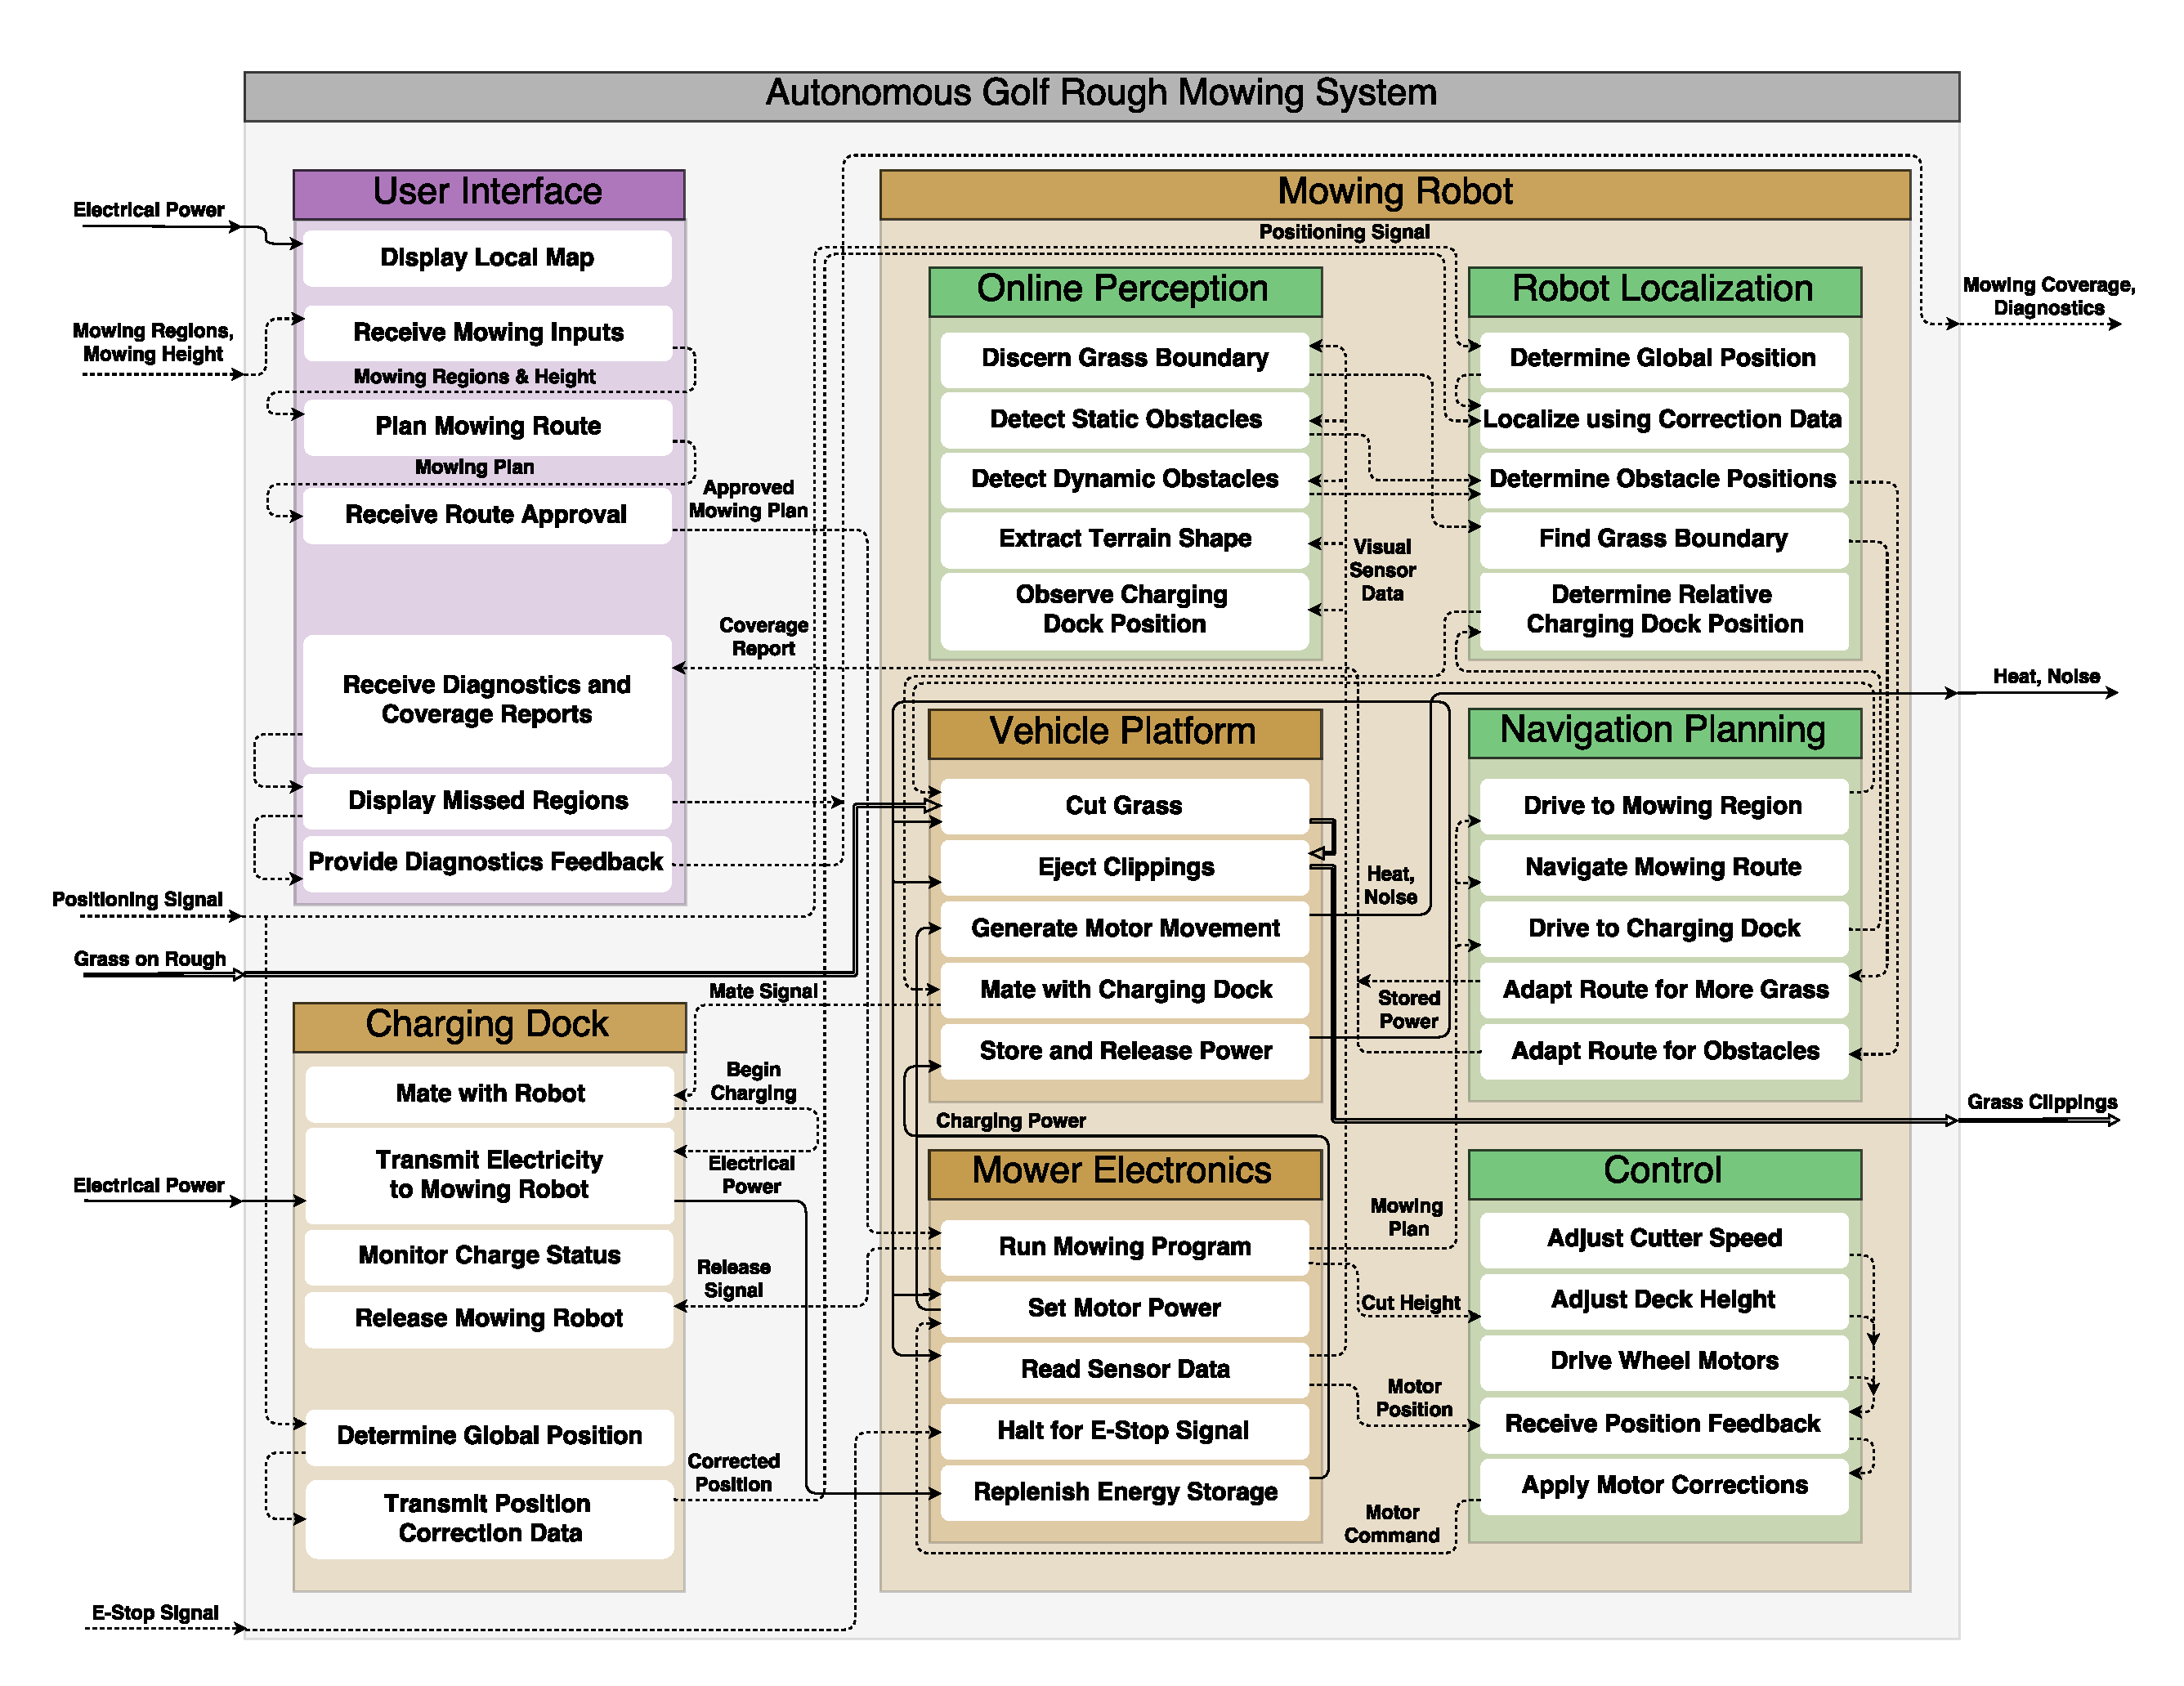
\includegraphics[scale=0.3]{functional}
\caption{Functional Architecture}
\label{fig:functional}
\end{figure}


\section{System Level Trade Studies}
	\subsection{Platform Trade Study}
		\begin{table}[H]
		\begin{adjustwidth}{-1.5in}{-1.5in}
		\centering
		\setlength{\dashlinedash}{.4pt}

		\begin{tabular}{|l|c|c|c|c|c|c|c|c|}
		\hline
		                                   & Speed & \makecell{Wheel \\ Compaction} & Stability & \makecell{Platform \\ Complexity} & \makecell{Odometry \\ Accuracy} & \makecell{Turning \\ Radius \\(Without tearing \\ the grass)} & \makecell{Performance \\ on Uneven \\ Terrain} & Score \\ \hline
		Weights (1-5)                      & 3     & 2                & 1         & 3                   & 4                 & 5                                          & 5                             &       \\ \hline
		4 Wheel Skid                       & 5     & 4                & 4         & 4                   & 1                 & 1                                          & 5                             & 73    \\ \hdashline 
		
		%jesus christ this row is a goddamn mess BUT YOU GOTTA DO WHAT YOU GOTTA DO
		\multicolumn{1}{|l|}{\cellcolor{lemonchiffon}\makecell[l]{2 wheel differential \\ with casters}}  & \multicolumn{1}{c|}{\cellcolor{lemonchiffon}4}     & \multicolumn{1}{c|}{\cellcolor{lemonchiffon}3}                & \multicolumn{1}{c|}{\cellcolor{lemonchiffon}4}         & \multicolumn{1}{c|}{\cellcolor{lemonchiffon}5}                   & \multicolumn{1}{c|}{\cellcolor{lemonchiffon}5}                 & \multicolumn{1}{c|}{\cellcolor{lemonchiffon}5}                               & \multicolumn{1}{c|}{\cellcolor{lemonchiffon}5}                             & \multicolumn{1}{c|}{\cellcolor{lemonchiffon}107}   \\ \hdashline
		
		\makecell[l]{4 Wheel Drive \\ Standard Steering}    & 5     & 4                & 4         & 2                   & 4                 & 2                                          & 5                             & 84    \\ \hdashline
		\makecell[l]{Rear Wheel Drive \\ Standard Steering} & 5     & 4                & 4         & 3                   & 5                 & 2                                          & 5                             & 91    \\ \hdashline
		Articulated                        & 3     & 4                & 2         & 1                   & 3                 & 2                                          & 5                             & 69    \\ \hdashline
		Tracked                            & 2     & 5                & 5         & 3                   & 1                 & 5                                          & 5                             & 84    \\ \hdashline
		3 Wheel Delta                      & 1     & 3                & 1         & 1                   & 1                 & 5                                          & 1                             & 47    \\ \hdashline
		4 Wheel Omniwheel                  & 2     & 4                & 2         & 1                   & 5                 & 5                                          & 1                             & 69    \\ \hline
		\end{tabular}
		\caption{Platform Configuration Trade Study}
		\label{my-label}
		\end{adjustwidth}
		\end{table}
		
		
		\begin{table}[H]
		\begin{adjustwidth}{-1.5in}{-1.5in}
		\centering
		\setlength{\dashlinedash}{.4pt}

		\begin{tabular}{|l|c|c|c|c|c|c|c|c|}
		\hline
		            & \makecell{Ease of \\ Integration} & \makecell{Ease of \\ Repair} & \makecell{Ease of \\ Construction} & \makecell{Flexiblility for \\ Modifications} & Cost & Leadtime & Traction & Score \\ \hline
		Weights (1-5)                      & 3                   & 2              & 3                    & 5                              & 3    & 2        & 4        &       \\ \hline
		\multicolumn{1}{|l|}{\cellcolor{lemonchiffon}Complete DIY} & \multicolumn{1}{c|}{\cellcolor{lemonchiffon}4}                   & \multicolumn{1}{c|}{\cellcolor{lemonchiffon}5}              & \multicolumn{1}{c|}{\cellcolor{lemonchiffon}2}                    & \multicolumn{1}{c|}{\cellcolor{lemonchiffon}5}                              & \multicolumn{1}{c|}{\cellcolor{lemonchiffon}4}    & \multicolumn{1}{c|}{\cellcolor{lemonchiffon}4}        & \multicolumn{1}{c|}{\cellcolor{lemonchiffon}5}        & \multicolumn{1}{c|}{\cellcolor{lemonchiffon}93}    \\ \hdashline
		RC Lawnmower                       & 5                   & 3              & 5                    & 4                              & 1    & 2        & 5        & 83    \\ \hdashline
		\makecell[l]{Modify Robot \\ Lawnmower}           & 3                   & 3              & 4                    & 1                              & 1    & 4        & 2        & 51    \\ \hdashline
		\makecell[l]{Modify Electric \\ Pushmower}         & 2                   & 2              & 3                    & 1                              & 2    & 5        & 1        & 44    \\ \hdashline
		\makecell[l]{Modify Electric \\ Ride on Mower}      & 2                   & 1              & 3                    & 1                              & 3    & 5        & 5        & 61    \\ \hdashline
		\makecell[l]{Stock platform with \\ mower attached} & 5                   & 3              & 5                    & 4                              & 1    & 3        & 3        & 77    \\ \hline
		\end{tabular}
		\caption{Platform Base Trade Study}
		\label{my-label}
		\end{adjustwidth}
		\end{table}

\section{Cyberphysical Architecture}
\begin{figure}[H]
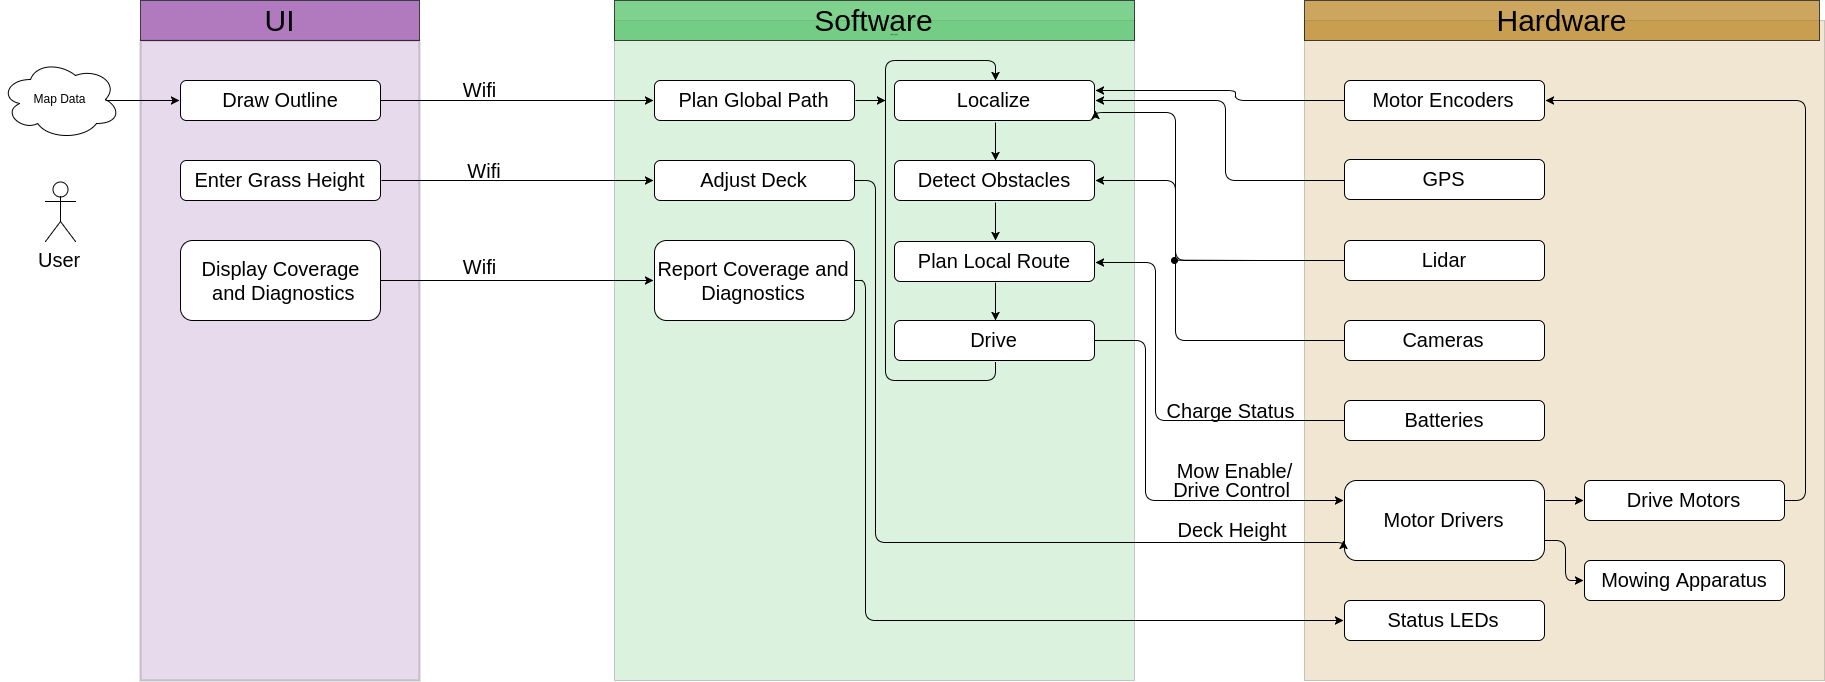
\includegraphics[scale=0.2]{cyberphysical}
\caption{Cyberphysical Architecture}
\label{fig:cyberphysical}
\end{figure}

  The user interface and IO subsystems are the contact points for the operator.  The wifi access point allows the user to load mowing boundaries from their laptop or mobile device.  This also enables the user to download coverage reports and diagnostics.  Status LEDs allow the operator to understand the system status at a glance, while safety beacons alert humans to GroundsBot's presence at a distance. \\

  GroundsBot uses its sensor suite to ensure a clean cut. GPS, IMU, and Motor Encoders are used for coarse localization while the cameras are used to ensure optimal grass overlap while cutting.  Cameras and lidar also enable GroundsBot to detect static and dynamic obstacles.\\

  GroundsBot's battery subsystem reports charge status to the CPU to prevent GroundsBot from becoming stranded. The battery subsystem also contains standard protection protocols including charge control, under-voltage lockout, and over-current protection. \\

  The CPU utilizes sensor information for localization, obstacle detection, and planning.  After a local path is devised drive signals are sent to the motors. The CPU also logs coverage data and generates reports.\\

  The Drive Train contains motors and motor drivers to propel GroundsBot across a golf course.  This also encompasses the mowing apparatus and mowing deck height control. \\



\section{Subsystem Descriptions}
	\subsection{UI}
	An important aspect of the project is a way for the user to communicate his desired mowing path to the robot. This input method must be separate from the robot itself, allowing the user to be somewhere else as the robot mows autonomously. 
	
	This will be achieved through a mobile device, either a dedicated tablet or the user's own smartphone. An app or website will be loaded onto this device, and allow for the user to input a map outline that will be communicated to the robot. 
	
	\subsection{Hardware}
		\subsubsection{Platform}
			Based on the trade study, a differential drive system with two drive wheels and one or more caster wheels will be used. Another trade study was used to narrow down the platform to DIY platform instead of a preexisting platform. This custom platform will utilize aluminum extrusions, allowing for easy resizing of the platform as well as easy adjustment of the sensor mounts. Currently, motors and batteries from Discovery Robotics will be integrated, but alternate products may be also be considered. 
			
		\subsubsection{Mower}
			In addition to navigating a plot of grass, the system also needs to mow it. Given that a custom platform will be made, this will be done by attaching an existing electric push mower to the robot platform. Alternatively, it is also possible to attach the blades from a manual reel mower to the platform. 
	
	\subsection{Software}
		\subsubsection{Planner}
			The planner subsystem consists of two parts, a global planner, and  a local planner. The global planner will take the user input from the UI, and translate that into a path that the robot will follow. This involves refining the outline that was provided by the user, and then finding a path that will allow for maximal coverage of the selected area. 
			
			The local planner will be responsible for adapting the route on-the-fly to avoid any obstacles that the robot may encounter. This system will also take care of the driving to and from the dock to the actual cutting area. 
			
		\subsubsection{Localization and Perception}
			An accurate description of the robot's global position and orientation will be obtained from this subsystem. This information may be obtained from a high-accuracy GPS system, such as RTK-GPS, but visual SLAM based methods will also be investigated. 
			
			The vision system will also be used to detect boundaries of the grass as the robot gets closer to the boundary. For obstacle detection, a trade study determined that a stereo camera system would best fit the detection requirements. However, if needed, a LIDAR may be added to improve the detection accuracy. 
		
		\subsubsection{Mobility}
			The mobility subsystem will be responsible for the control of the robot's motors. Part of this involves the robot going from point A to point B at any given time. Using current position information from localization subsystem, this subsystem will find the next waypoint that will allow for the robot to follow the predetermined plan and then emit the necessary motor control signals to move towards this waypoint. 
			
			The cutter motor speeds will also be controlled by this subsystem. This subsystem must both detect the speed of the motor, as well as apply the correct motor signals to maintain a constant speed when the cutter encounters an obstacle. 


\section{Project Management}
\subsection{Work Plan}
\subsubsection{Tasks}
The GroundsBot work plan is shown in the list below.  The plan is separated into high level categories and underlying subtasks. \\
\begin{outline}[enumerate]
  \1 Chassis
    \2 Complete BOM
    \2 Design Power Distribution and Sensor Integration PCBAs
    \2 Design Chassis
    \2 Design GPS RTK Base Station
    \2 Acquire Parts
    \2 Integrate Subsystems
  \1 Simulation
    \2 Design Simulation Environment
    \2 Complete Cursory Simulations
  \1 Localization
    \2 Integrate GPS + RTK Localization
  \1 Perception
    \2 Develop Static Obstacle Detection
    \2 Develop Dynamic Obstacle Detection
  \1 Planning
    \2 Develop Global Route Planner
    \2 Develop Obstacle Rerouting
  \1 Control
    \2 Develop Motor Control
  \1 UI
    \2 Create Web Application for Mapping
\end{outline}

   
\subsubsection{Schedule}
\textbf{Progress Review 1}: The goal for Progress Review 1 is to have all hardware design complete with parts on order. \\
\textbf{Progress Review 2}: The goal for Progress Review 2 is to have an assembled frame/chassis, a full ROS simulation environment, and a completed GPS + RTK base station\\

The full list of milestones is laid out below in Table \ref{Tab:table_milestones}\\ 

\begin{table}[H]
\begin{tabular}{|l|l|}
\hline
Deadline & Milestone                            \\
\hline
Progress Review 1 [OCT 17 2017] &
  \makecell[l]{
    Mechanical CAD Complete                     \\
    Electrical CAD Complete                     \\
    BOM Complete                                \\
    Parts Ordered                               \\
    ROS Environment Initialized                 \\
  }                                             \\
  \hline
Progress Review 2 [OCT 26 2017] &
  \makecell[l]{
    Chassis Assembled with Mowing Apparatus     \\
    ROS Simulation Environment Complete         \\
    GPS RTK Base Station Complete               \\
  }                                             \\ 
  \hline
Progress Review 3 [NOV 7 2017] &
  \makecell[l]{
    GroundsBot System Integration Complete      \\
    GPS RTK Integration Complete                \\
    Control Systems Demo Complete               \\
  }                                             \\
  \hline
Progress Review 4 [NOV 21 2017] &
  \makecell[l]{
    GroundsBot Accepts GPS Waypoints            \\
    GroundsBot Follows GPS waypoints            \\
    Teleoperation Test Complete                 \\
  }                                             \\
  \hline
Fall Validation Experiment [NOV 28 2017] &
  \makecell[l]{
    GroundsBot Follows Route From Web App       \\
    GroundsBot Differentiates Grass From Other Objects
  }                                             \\
  \hline
January 2018 Milestone &
  \makecell[l]{
    Global Planning Algorithm Complete          \\
    Static and Dynamic Obstacle Detection Complete\\
  }                                             \\
  \hline
February 2018 Milestone &
  \makecell[l]{
    Read User Map Input                        \\
    GroundsBot Reroutes Around Obstacles       \\
  }                                            \\
  \hline
March 2018 &
  \makecell[l]{
    Full Mapping UI Complete                   \\
    GroundsBot Autonomously Cuts Lot           \\
  }                                            \\
  \hline
April 2018 &
  \makecell[l]{
    Final System Tests Complete                \\
  }                                            \\
  \hline
\end{tabular}
\caption{Project Milestones}\label{Tab:table_milestones}
\end{table}

\subsubsection{Progress Reviews}

\subsection{System Validation Experiments}
\subsubsection{Fall Validation Experiment}
Fall Validation
Location: Field by Doherty Apartments
\subsubsection{Spring Validation Experiment}

\subsection{Team Member Responsibilities}
\subsection{Provisional BOM}
\begin{center}
\begin{tabular}{ |c|c|c|c|c| }
  \hline
    Manufacturer & Part No. & QTY & Description & Notes \\
    \hline 
    Murata & C1 & 10 & my capacitor &  \\
  \hline
\end{tabular}
\end{center}

\subsection{Risk Management}
\section{References}

\end{document}
